\documentclass[12pt]{article}

\usepackage{times}
\usepackage{amsmath}
\usepackage{url}
\usepackage[pdftex]{graphicx}

\usepackage{rotating}

\begin{document}
	
\section{Summary of Changes}
\subsection{Changes in PAM~3.0}
\label{sec:changes-2.0}
We built a new web application using Shiny. We have written instructions on how to use this new application. Results we get from running PAM remains the same as the previous version. PAM no longer accepts .xls file. Please convert the data into .xlsx before running SAM.
	
\section{Running PAM: Classification Problems}
Download the pamr package in R. Load in pamr library and type in {\tt runPAM()} to run PAM.
Once the PAM interface is up, upload an .xlsx data file by clicking on the {\tt Choose File} button. Note .xls
file will not work any more. The data has to follow the format specified.

Then, you need to enter the row number that contains the class labels and the row number that indicates
the start of an expression data. You also need to include the row numbers for sample labels and batch labels
if you have those included in your dataset. Figure below shows an example of how this is done for the example file
{\tt khan.xlsx}. Once these information has been put in, the program automatically displays your dataset
under the {\tt Data} tab. You can change
parameters and press tabs (Training, Cross Validation, etc) to view analysis results.
Changes in the parameters, such as threshold changes the result interactively.
 
To save the results in excel, you need to specify where you want to save and what you want
to name the file and press the {\tt Save} button. The default is the current directory and 
a file name called \emph{result}. It takes a few seconds to save plots and tables
in an excel format. Note that if there is already an excel file with the same name, the previous 
file is replaced with a new file. If you have any missing data in your data, a new worksheet named
{\tt Imputed Data} containing the imputed dataset is added
to the workbook. This data can be used in subsequent analyses to save
time. If there is no missing data, this worksheet is not added.

\begin{sidewaysfigure}[htbp]
  \leavevmode
  \begin{center}
    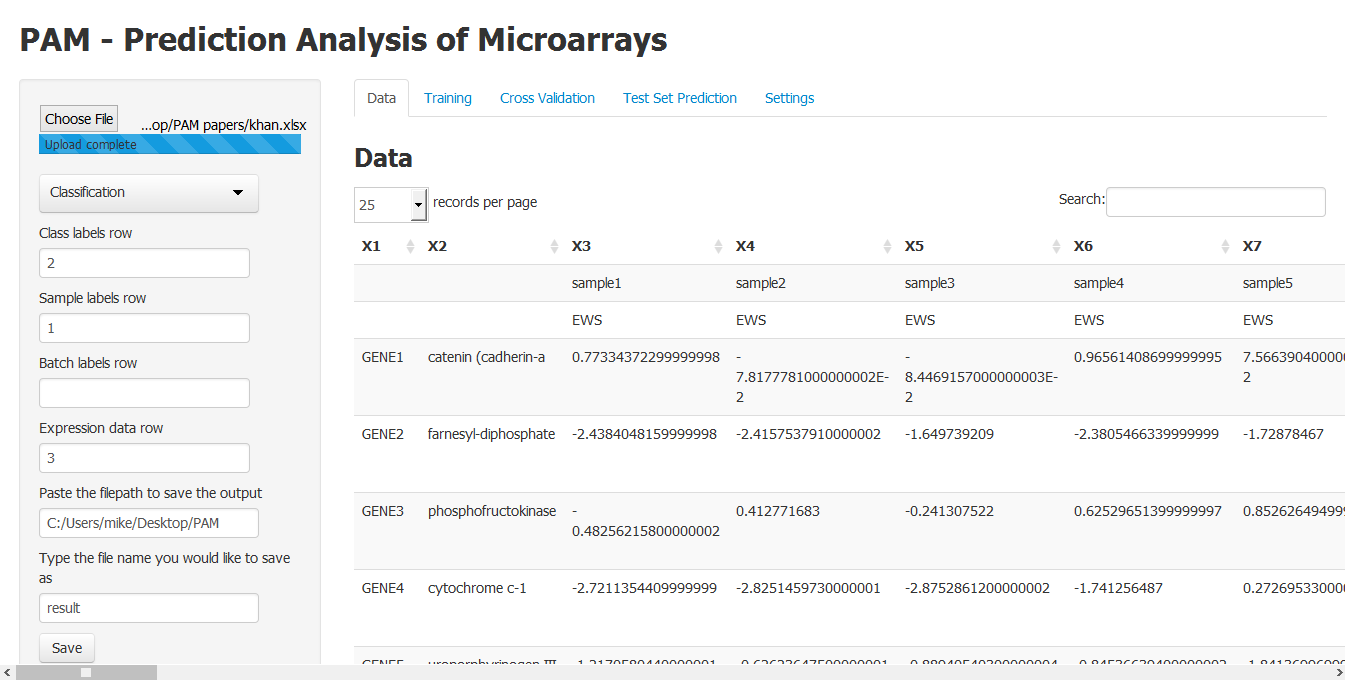
\includegraphics[width=1\textwidth]{pam1.png}    
    \caption{How to start PAM running}
    \label{fig:pam-start}
  \end{center}
\end{sidewaysfigure}


\begin{figure}[htbp]
  \begin{center}
    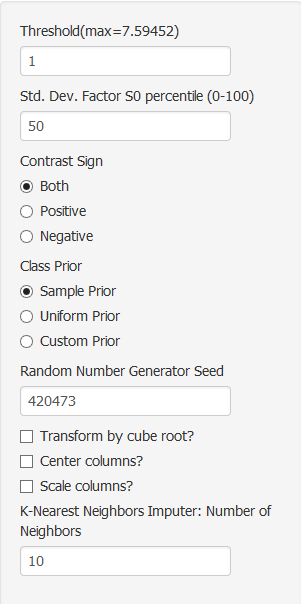
\includegraphics[width=0.5\textwidth]{pam2.png}    
    \caption{PAM parameters to change}
    \label{fig:pam-parameters}
  \end{center}
\end{figure}

\begin{sidewaysfigure}[htbp]
  \begin{center}
    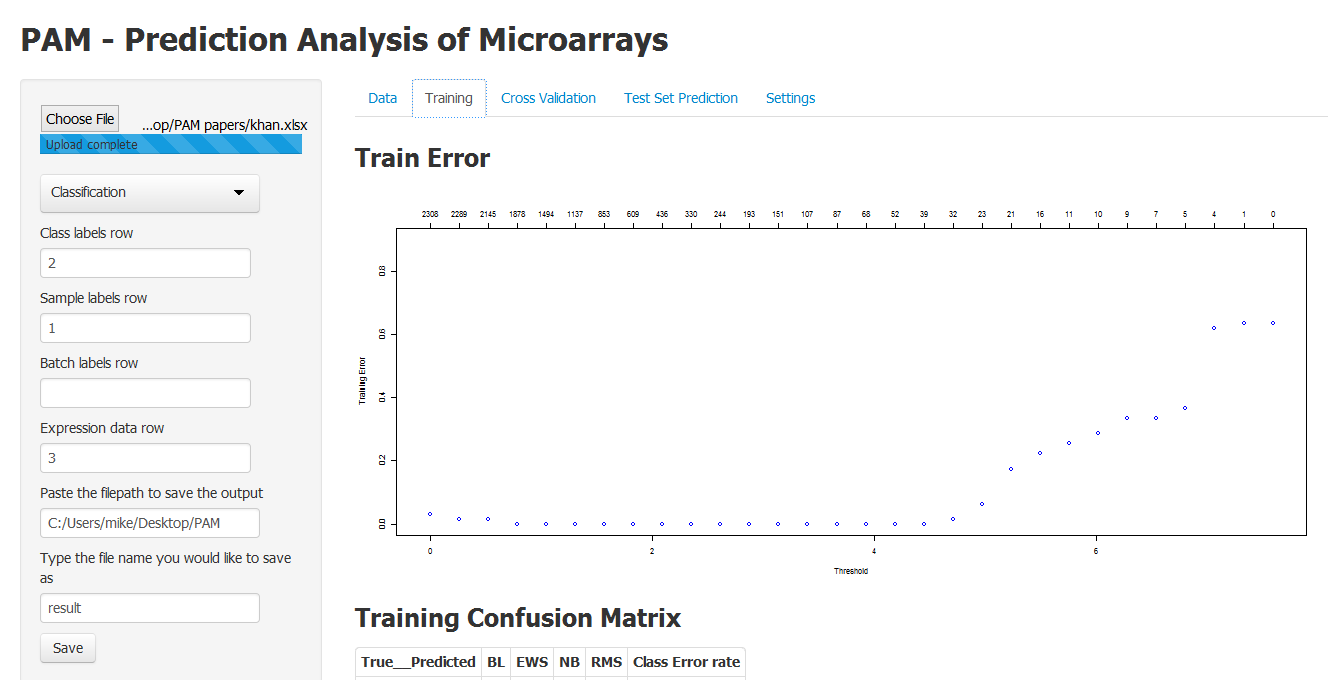
\includegraphics[width=1\textwidth]{pam3.png}    
    \caption{PAM Results}
    \label{fig:pam-results}
  \end{center}
\end{sidewaysfigure}

\newpage
\section{Running Survival analysis and regression}

For survival analysis problems, you are asked for Survival Time and Censoring Status instead
of Class Labels. For regression analysis problems, you will be asked for the Outcome variable.
Sample labels are not required in general, but are required if a comparison to competing predictors
is desired. Figure FILL shows the format of competing predictors in excel.

\begin{figure}[htbp]
	\begin{center}
		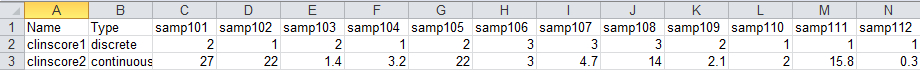
\includegraphics[width=1\textwidth]{pam4.png}    
		\caption{Competing Predictors Format}
		\label{fig:pam-parameters}
	\end{center}
\end{figure}


\end{document}